\section{Specification}
The following chapter describes the implementation of the application.
\subsection{Main window}
The main window is divided into two parts, see figure \ref{fig:mainwindow}. On the very top of the application is a menubar where the user can do actions like saving their work. Then the window is split up in two parts. On the left side is the menubar and on the right side the grid. The grid is the representation of the traffic situation. The components (see section \ref{sec:components}) can be dragged from the sidebar to the grid. To remove a component right-click on it and press on Delete in the context-menu. All open incoming lanes have a text-box which allows the user to specify the amount of traffic coming. The simulation can simply be started by the play button and the simulation speed can simply be changed with a slider. With the button "Show Report" the user can get a report of that moment of the simulation. The report will contain a still image of the current situation. It highlights the traffic jams and the image can be saved.

\begin{figure}[!ht]
	\caption{Mockup of the Main window}
	\label{fig:mainwindow}
	\centering
	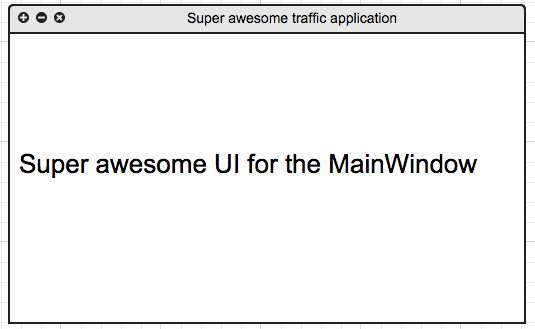
\includegraphics[width=0.8\textwidth]{figures/mainwindow}
\end{figure}
\begin{tabularx}{\textwidth}{|p{2cm}X|}\hline
	Code & Specification \\\hline
	MWS-010 & When the application just started it will create a new grid 4x3\\\hline
	MWS-020 & The main window has a menubar.\\\hline
	MWS-020A & The menu bar has the following structure:
	\begin{itemize}[noitemsep,nolistsep]
		\item File
		\begin{itemize}
			\item New
			\item Open
			\item Save
			\item Save As
		\end{itemize}
		\item Help
	\end{itemize}\\\hline
	MWS-020B & A new simulation can be started by pressing on new, a window will prompt for the width and height for the size of the grid.\\\hline
	MWS-020C & The manual can be opened by pressing on Help.\\\hline
	MWS-030 & The window has a sidebar on the left.\\\hline
	MWS-032 & The sidebar contains all the components described in section \ref*{sec:components}.\\\hline
	MWS-032A & The component can be added to the grid by dragging it to the desired location.\\\hline
	MWS-034 & The sidebar contains a button which allows the simulation to start/stop.\\\hline
	MWS-035 & The sidebar contains a button which allows the simulation to pause.\\\hline
	MWS-036 & The simulation-speed can be changed by adjusting the slider.\\\hline
	MWS-038 & In simulation the button "Show report" will generate a report.\\\hline
	MWS-038A & The report is shown in a new window and contains the current traffic situation including cars and pedestrians.\\\hline
	MWS-038B & In the report the traffic jams are highlighted.\\\hline
	MWS-038C & The report can be saved as an image file.\\\hline
\end{tabularx}

To change the amount of time each traffic light is green press right-click on the crossway and click in the context-menu on "Traffic-light configuration". A new window will pop up which allows to set the time for each group of lanes.

\begin{tabularx}{\textwidth}{|p{2cm}X|}\hline
	Code & Specification \\\hline
	MWS-100 & All open incoming lanes have a textbox to specify the amount of traffic coming in.\\\hline
	MWS-110 & When pressing right-click on any component placed on the grid a context-menu appears which allows to rotate or delete the component.\\\hline
	MWS-120 & When pressing right-click on a crossway it gives an option "Traffic-light configuration"\\\hline
	MWS-120A & A new window will pop-up with a list of all the lane groups.\\\hline
	MWS-120B & The user can select a lane group and change the amount of time the traffic-light is green.\\\hline
\end{tabularx}

\newpage
\subsection{Components}
\label{sec:components}
\subsubsection{Crossway}
\begin{figure}
	\centering
	\begin{subfigure}{.5\textwidth}
		\centering
		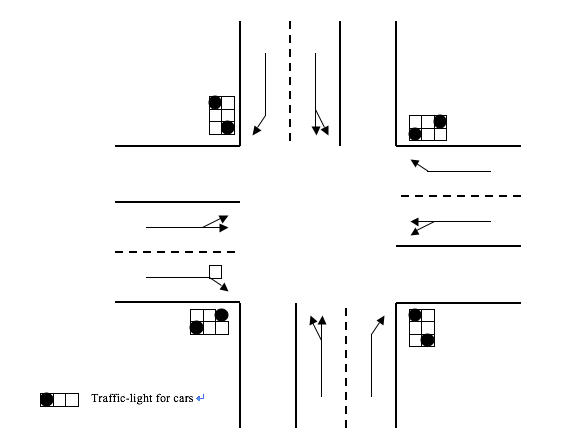
\includegraphics[width=\linewidth]{figures/crosswaya.png}
		\caption{Crossway without pedestrians.}
		\label{fig:crossa}
	\end{subfigure}%
	\begin{subfigure}{.5\textwidth}
		\centering
		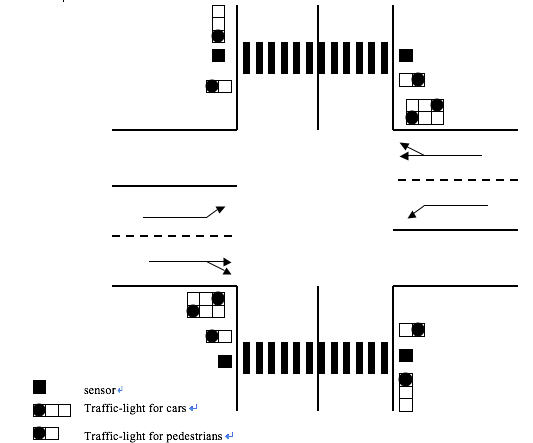
\includegraphics[width=\linewidth]{figures/crosswayb.png}
		\caption{Crossway with pedestrians.}
		\label{fig:crossb}
	\end{subfigure}
	\caption{Crossways}
	\label{fig:cross}
\end{figure}

\begin{tabularx}{\textwidth}{|p{2cm}X|}\hline
	Code & Specification \\\hline
	CWC-010 & All cossways are connected to 4 roads\\\hline
	CWC-020 & There are 2 different types of crossways see figure \ref{fig:cross}.\\\hline
	CWC-020 & Type A crossway is without pedestrian lane.\\\hline
	CWC-020A & From each side the crossway A has 2 incoming lanes and 1 outgoing lane.\\\hline
	CWC-025 & Type B crossway is with an pedestrian lane.\\\hline
	CWC-025A & Type B has from 2 opposite sides a crossway for pedestrians, which only has 1 incoming lane.\\\hline
	CWC-030 & Traffic light for cars have the colors red, orange and geen.\\\hline
	CWC-035 & Traffic light for pedestrians have the colors red and green.\\\hline
	CWC-040 & Traffic light for cars only turn orange after green.\\\hline
	CWC-040A & Amount of time for the orange light is fixed, and is set to 2 seconds in normal simulation time.\\\hline
	CWC-045 & Traffic light for green are set to default for 4 seconds.\\\hline
	CWC-045A & The amount of time each light group of an crossway can be changed.\\\hline
	CWC-050 & The order of the light groups are fixed.\\\hline
	CWC-050A & When there are no cars or pedestrians on the sensors for the according lightgroup it will be skipped in the simulation.\\\hline
\end{tabularx}

\subsubsection{Road}
\begin{figure}
	\centering
	\begin{subfigure}{.5\textwidth}
		\centering
		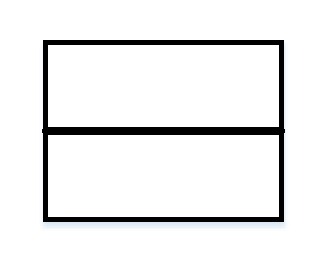
\includegraphics[width=\linewidth]{figures/straightroad.pdf}
		\caption{Crossway without pedestrians.}
		\label{fig:crossa}
	\end{subfigure}%
	\begin{subfigure}{.5\textwidth}
		\centering
		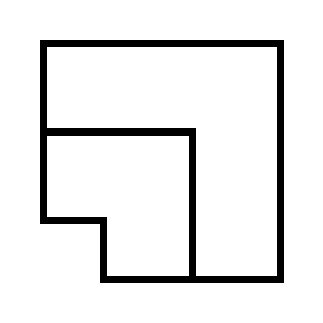
\includegraphics[width=\linewidth]{figures/curvedroad.pdf}
		\caption{Crossway with pedestrians.}
		\label{fig:crossb}
	\end{subfigure}
	\caption{Crossways}
	\label{fig:cross}
\end{figure}

\subsection{Traffic light groups}
\textsl{At the moment of writing this document it is unclear what the traffic light groups are.}
